\chapter{Realization of Intention-centric Organizational Modeling}
\label{chap:realization}
\hspace{4ex} This chapter discusses about how Intention-centric organizational modeling realized as an user interface editor. This also explains the realization of requirements described in Chapter 4. In the first section, we will first discuss the overview of basic concepts and then specify the design components required for the realization of this editor. The next section discusses about how the entity views in particular are realized. The last section covers in detail how individual requirement has been realized through the web editor.


%%%%%%%%%%%%%%%%%%%%%%%%%%%%%%%%%%%%%%%%%%%%%%%%%%%%%%%%%%%%%%%%%%%%%%%%%
\section{Basic Concepts}
%%%%%%%%%%%%%%%%%%%%%%%%%%%%%%%%%%%%%%%%%%%%%%%%%%%%%%%%%%%%%%%%%%%%%%%%%
\hspace{4ex} The basic concepts section provides an overview about the architectural details like design patterns and frameworks of the developed web editor.
%%%%%%%%%%%%%%%%%%%%%%%%%%%%%%%%%%%%%%%%%%%%%%%%%%%%%%%%%%%%%%%%%%%%%%%%%
\subsection{MVC Architecture}
%%%%%%%%%%%%%%%%%%%%%%%%%%%%%%%%%%%%%%%%%%%%%%%%%%%%%%%%%%%%%%%%%%%%%%%%%
\hspace{4ex} The architecture of the UI editor is based on the \textbf{Model-View-Control (MVC)} design pattern. The MVC paradigm allows to separate business logic from the code that controls presentation and event handling \cite{Oracle2016}.Each entity view in the web page is made up of combination of at least on Model and View, and one or more Controls. The individual files which acts an Model, View and Controller has been shown in the Figure \ref{fig:mvc_arch}

\begin{itemize}
	\item \textbf{Model} artifact stores the required data structure for web-editor. In the developed model artifact, the four main types of data stored inside the artifact are intentions, strategies, capabilities and informal process instances. 
	\item \textbf{View} artifact contains HTML elements and HTML constructs that describe the way of displaying the data from Model to the user.
	\item \textbf{Control} artifact contains the handler functions which can only change the model. Even the initial values of the model are put inside the control. 
\end{itemize}


\begin{figure}
	\centering
	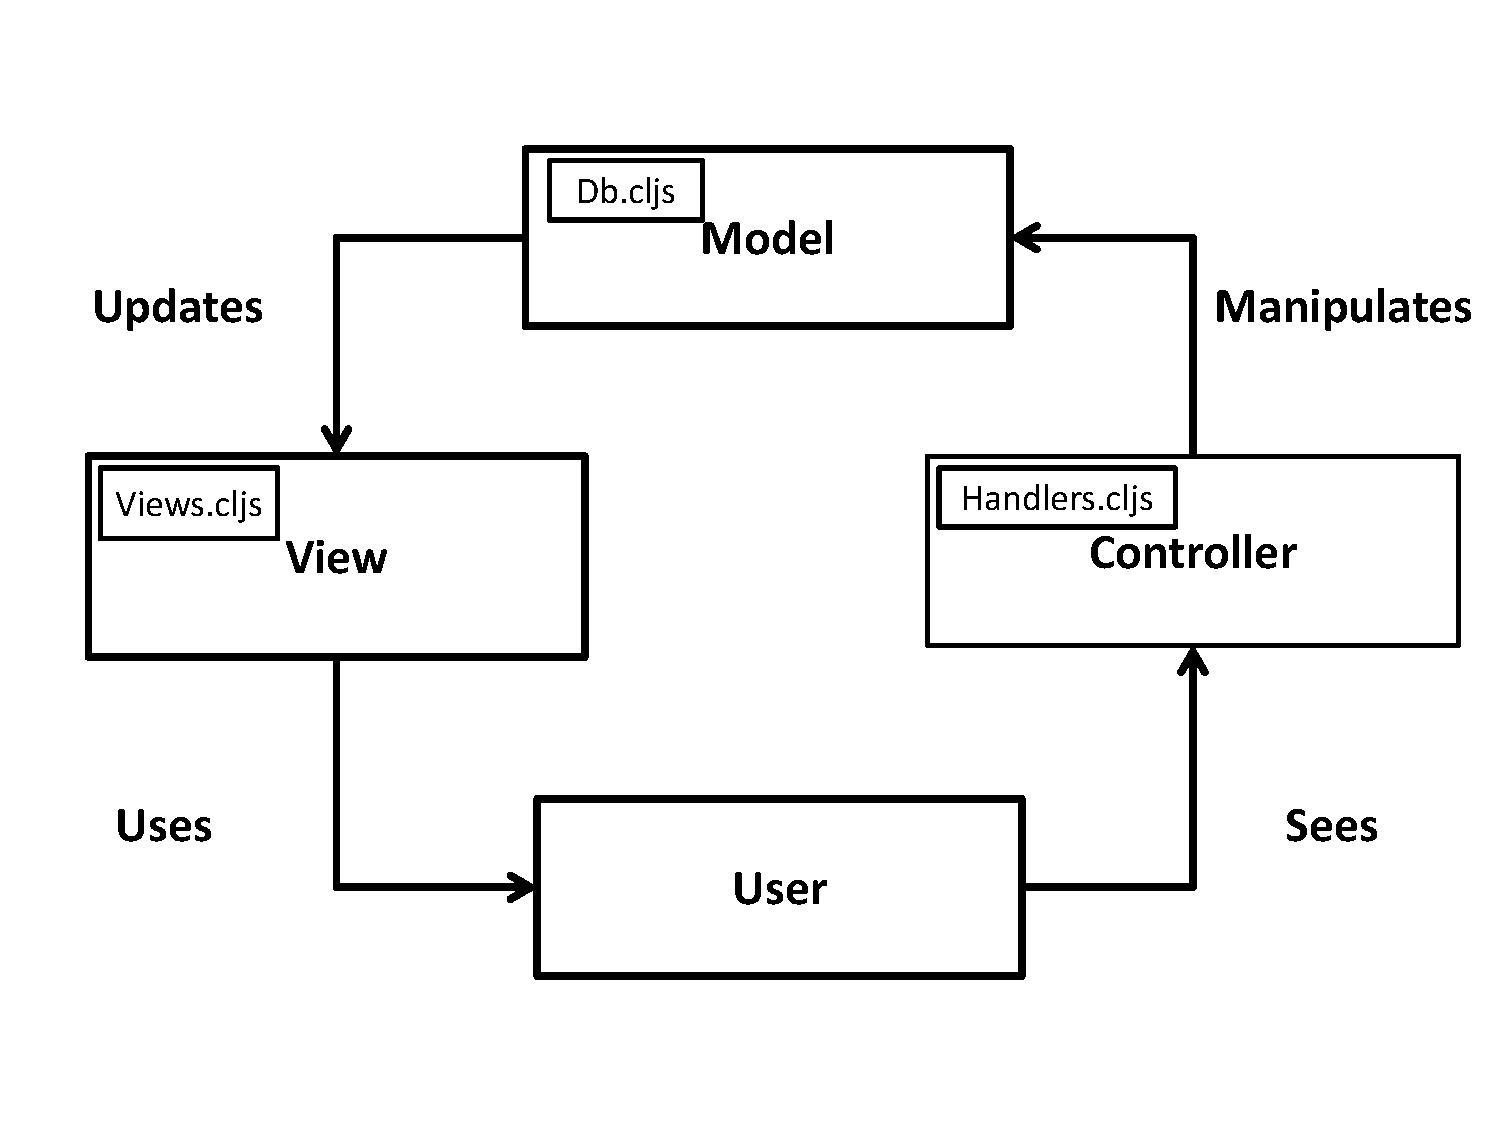
\includegraphics [width= 0.75\textwidth]{mvc_arch.pdf}
	\caption{Relationship between developed web editor artifacts and MVC architecture components}
	\label{fig:mvc_arch}
\end{figure}

 
%%%%%%%%%%%%%%%%%%%%%%%%%%%%%%%%%%%%%%%%%%%%%%%%%%%%%%%%%%%%%%%%%%%%%%%%%
\subsubsection{Example: Component using MVC Pattern }
%%%%%%%%%%%%%%%%%%%%%%%%%%%%%%%%%%%%%%%%%%%%%%%%%%%%%%%%%%%%%%%%%%%%%%%%%
\hspace{4ex} The Figure \ref{fig:mvc_arch} below shows the simplifed version of how the components interact with each other using the Model-View-Control (MVC) pattern, for the functionality adding new entity data. This functionality is same for all the types intentions, strategies, capabilities and informal proceess instances and below is the detailed explanation of each interaction.

\begin{enumerate}
\item User clicks the tab \textbf{Add New} in the web editor.
 \item View, in response to the user click displays the UI component for entering the new entity data details.
\item User enters the required basic details for adding new entity data and clicks save button.
 \item View dispatches the data to Control, which can only modify the Model.
\item Control inserts/updates data into the model.
\item View displays the updated model as it has been subscribed to the model.
\end{enumerate}

\begin{figure}
	\centering
	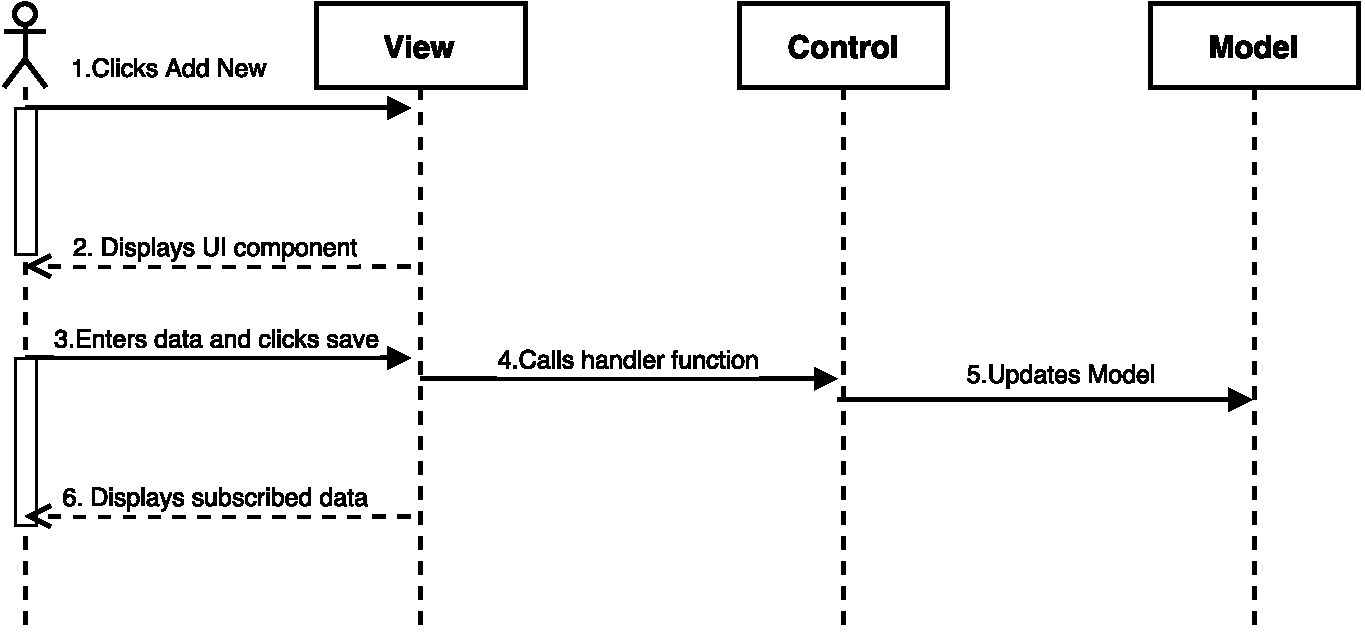
\includegraphics [width= \textwidth]{mvc_pattern.pdf}
	\caption{MVC Pattern of adding new entity}
	\label{fig:mvc_pattern}
\end{figure}
%%%%%%%%%%%%%%%%%%%%%%%%%%%%%%%%%%%%%%%%%%%%%%%%%%%%%%%%%%%%%%%%%%%%%%%%%
\subsection{Flux Architecture}
%%%%%%%%%%%%%%%%%%%%%%%%%%%%%%%%%%%%%%%%%%%%%%%%%%%%%%%%%%%%%%%%%%%%%%%%%

\cite{Flux2016}
%%%%%%%%%%%%%%%%%%%%%%%%%%%%%%%%%%%%%%%%%%%%%%%%%%%%%%%%%%%%%%%%%%%%%%%%%
\subsection{Using Reagent Framework}
%%%%%%%%%%%%%%%%%%%%%%%%%%%%%%%%%%%%%%%%%%%%%%%%%%%%%%%%%%%%%%%%%%%%%%%%%
 
\cite{Reframe2016}

\begin{figure}
	\centering
	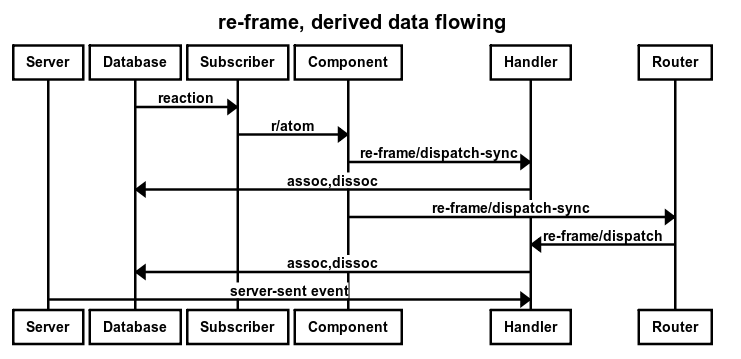
\includegraphics [width= 0.75\textwidth]{reframe_dataflow.png}
	\caption{Reframe, derived data flowing}\cite{Reframe2016a}
	\label{fig:reframe_dataflow}
\end{figure}



%%%%%%%%%%%%%%%%%%%%%%%%%%%%%%%%%%%%%%%%%%%%%%%%%%%%%%%%%%%%%%%%%%%%%%%%%
\section{Specifications}
%%%%%%%%%%%%%%%%%%%%%%%%%%%%%%%%%%%%%%%%%%%%%%%%%%%%%%%%%%%%%%%%%%%%%%%%%



%%%%%%%%%%%%%%%%%%%%%%%%%%%%%%%%%%%%%%%%%%%%%%%%%%%%%%%%%%%%%%%%%%%%%%%%%
\section{Realization of Entity Views}
%%%%%%%%%%%%%%%%%%%%%%%%%%%%%%%%%%%%%%%%%%%%%%%%%%%%%%%%%%%%%%%%%%%%%%%%%


%%%%%%%%%%%%%%%%%%%%%%%%%%%%%%%%%%%%%%%%%%%%%%%%%%%%%%%%%%%%%%%%%%%%%%%%%
\section{Realization of Requirements}
%%%%%%%%%%%%%%%%%%%%%%%%%%%%%%%%%%%%%%%%%%%%%%%%%%%%%%%%%%%%%%%%%%%%%%%%%